\documentclass[12pt,a4paper]{article}

\usepackage[T1]{fontenc}
\usepackage[brazilian]{babel}
\usepackage{lmodern}
\usepackage[margin=2.5cm]{geometry}
\usepackage{amsmath}
\usepackage{amssymb}
\usepackage{graphicx}
\usepackage{booktabs}
\usepackage{microtype}
\usepackage{natbib}
\usepackage[hidelinks]{hyperref}

\title{Relatório de Análise da Qualidade do Ar: Ozônio}
\author{Diego Lopes Vieira}
\date{\today}

\begin{document}

\maketitle

\section{Introdução e Dados}
\label{sec:introducao}

O conjunto de dados analisado neste relatório reúne medições diárias de parâmetros de qualidade do ar em Nova York entre maio e setembro de 1973, disponibilizado originalmente no pacote básico do software estatístico R \citep{rcore}. A base de dados conta com um total de 153 observações diárias distribuídas ao longo de cinco meses consecutivos.

A variável selecionada para a análise é a concentração de ozônio (\textit{Ozone}), expressa em partes por bilhão (ppb). Dentre as 153 observações registradas no arquivo, identificou-se que 37 valores são faltantes (\texttt{NA}). O processamento estatístico e a geração dos relatórios gráficos seguiram convenções modernas de reprodutibilidade computacional, cuja estrutura tipográfica e de compilação em \LaTeX{} fundamenta-se nos princípios descritos por \citet{lamport1994}.

\section{Resultados e Análise Mensal}
\label{sec:resultados}

A média amostral da concentração de ozônio para cada mês $m$, denotada por $\bar{Y}_m$, é calculada de acordo com a Equação~\eqref{eq:media},
\begin{equation}
  \label{eq:media}
  \bar{Y}_m = \frac{1}{n_m} \sum_{i=1}^{n_m} Y_{mi},
\end{equation}
em que $Y_{mi}$ representa a $i$-ésima medição válida no mês $m$. Na Equação~\eqref{eq:media}, o denominador $n_m$ contabiliza exclusivamente o número de dias efetivamente medidos naquele mês, desconsiderando os dias com valores ausentes (\texttt{NA}), e não o número total de dias do calendário.

Conforme apresentado na Tabela~\ref{tab:resumo}, as médias mensais de ozônio sofrem forte elevação durante os meses mais quentes do verão nova-iorquino (julho e agosto), atingindo patamares próximos a 60,0~ppb, em comparação aos meses de primavera e transição para o outono.

\begin{table}[htbp]
  \centering
  \caption{Médias mensais da concentração de ozônio e total de dias medidos.}
  \label{tab:resumo}
  \begin{tabular}{lrr}
    \toprule
    Mês & Dias medidos ($n_m$) & Média de Ozônio (ppb) \\
    \midrule
    Maio     & 26 & 23,6 \\
    Junho    &  9 & 29,4 \\
    Julho    & 26 & 59,1 \\
    Agosto   & 26 & 60,0 \\
    Setembro & 29 & 31,4 \\
    \bottomrule
  \end{tabular}
\end{table}

A distribuição completa da concentração de ozônio e sua variabilidade ao longo dos cinco meses podem ser visualizadas na Figura~\ref{fig:distribuicao}, gerada a partir do script R. Observa-se maior dispersão e a ocorrência de valores extremos durante os meses de julho e agosto, o que corrobora os valores médios tabulados.

\begin{figure}[htbp]
  \centering
  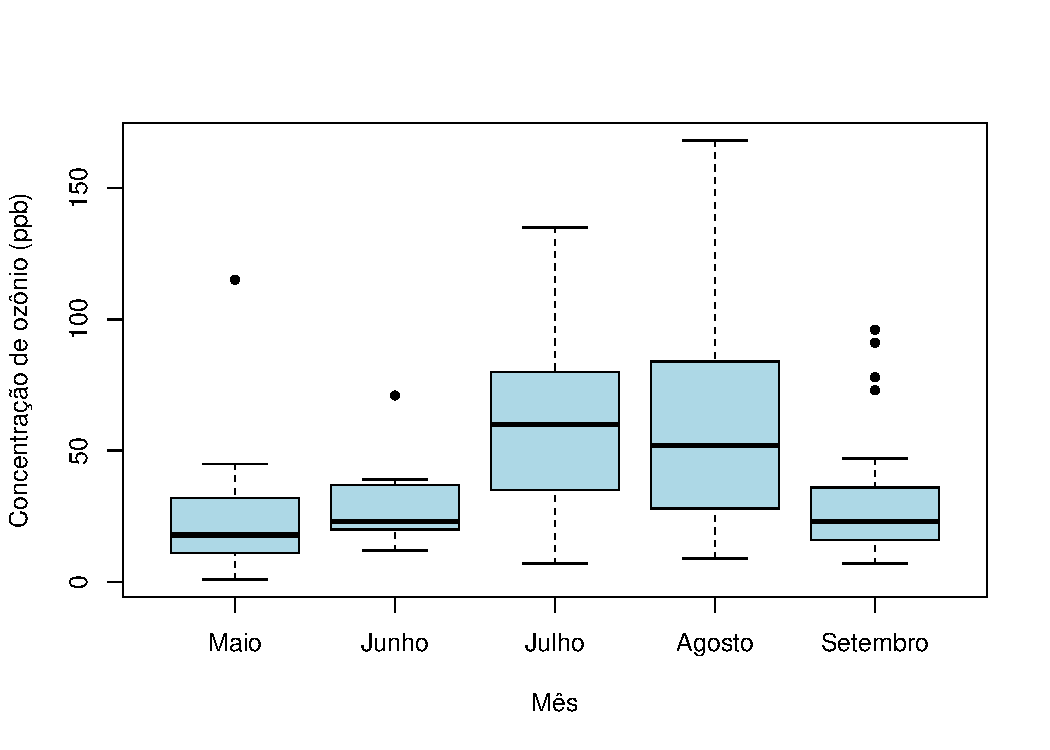
\includegraphics[width=0.75\textwidth]{figura.pdf}
  \caption{Distribuição da concentração de ozônio (ppb) por mês em Nova York.}
  \label{fig:distribuicao}
\end{figure}

\section*{Declaração de uso de IA}

Utilizou-se o assistente Antigravity (baseado no modelo Gemini, Google DeepMind) como ferramenta de apoio para consulta de sintaxe \LaTeX{}, redação do preâmbulo e dos comandos de terminal. Todas as análises numéricas, linhas de código em shell script, comandos do R e arquivos gerados foram inspecionados, executados e validados localmente no terminal.

\bibliographystyle{plainnat}
\bibliography{referencias}

\end{document}
